% ----- Compilar pdflatex -> pdflatex
\documentclass[12pt]{article}

\usepackage[utf8]{inputenc}
\usepackage[portuges]{babel}
\usepackage{multirow}
\usepackage{booktabs}
\usepackage[a4paper]{geometry}
\usepackage{amsmath}
\usepackage{graphicx}
\usepackage{float}
\usepackage{natbib}
\usepackage{hyperref} 
\usepackage{indentfirst}
\usepackage{xcolor}
\definecolor{dark-red}{rgb}{0.4,0.15,0.15}
\definecolor{dark-blue}{rgb}{0.15,0.15,0.5}
\definecolor{medium-blue}{rgb}{0,0,0.5}

\hypersetup{
  colorlinks, linkcolor={dark-blue},
  citecolor={medium-blue}, urlcolor={dark-red}
}

% opening
\title{Distribuição Gamma}
\author{Bruno Normande}
\date{\today}

\begin{document}

\maketitle

\section{Algumas características}

A distribuíção Gamma é uma distribuíção que é caracterizda por dois
parâmentros, \textit{shape} ($k$) e \textit{scale} ($\theta$). Ela
possui a seguinte função densidade probabilidade:

\begin{align}
  f(w;k,\theta) & =
  \frac{w^{k-1}e^{\frac{w}{\theta}}}{\theta^k\Gamma(w)}
  \intertext{para}
  k,\theta > 0
\end{align}

Essa distribuição é usada muitas vezes para modelar o tempo de espera,
como por exemplo em teste de vida a distribuição Gamma é usada para
modelar o tempo até a morte. A figura \ref{fig:densidade} mostra o
comportamento de Gamma para diferentes valores de $k$ e $\theta$.

\begin{figure}[h!]
  \centering
  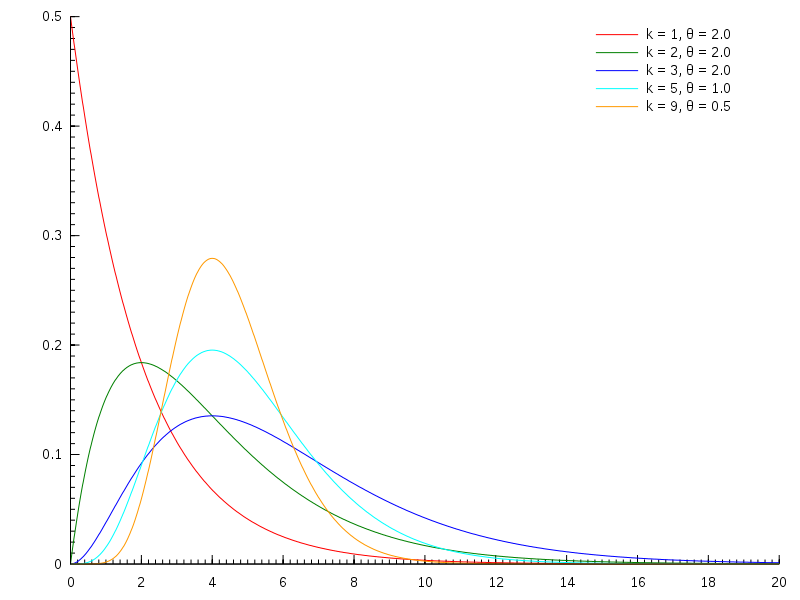
\includegraphics[width=.8\textwidth]{gamma_distribution.png}
  \caption{Função probabilidade Densidade de Gamma para diferentes parâmetros}
  \label{fig:densidade}
\end{figure}

Obtemos a esperança e a variância da distribuição com as seguintes
fórmulas:

\begin{align}
  E[W] &= k\theta\\
  Var[W] &= k\theta^2
\end{align}


\section{Estimadores}

Nesse trabalho foram analisados 6 estimadores para a distribuição
Gamma. Em todos foi usado $\theta = 1$ para manter a simplicidade dos
teste. Os estimadores usados foram:

\subsection{Estimador por Máxima Verossimilhança}

  Para estimar pela Máxima Verossimilhança é preciso maximizar a
  sua função log-verossimilhança de $\Gamma(w;k,1)$

  \small \begin{align}
%    \label{eq:Gamma_MV}
    log(p(W|k,1)) &= n(k-1)\overline{log(x)} - n log(\Gamma(k)) - n k
    log(\overline{x}) +  n k log(a) - n k
    \intertext{Que podemos resolver numericamente iterando sobre k em:}
%    log(p(W|k,1)) &\approx c_0 + c_1a + c_2log(a)
    \frac{1}{k} &= \frac{1}{k_0} + \frac{\overline{log(x)} -
      log(\overline{x}) + log(k_0) - \psi(k_0)}{k_0^2 (\frac{1}{k_0} -
      \psi'(k_0))} \\
    \intertext{até o momento em que}
    k &\approx k_0 \\
    \intertext{Como k inicial podemos usar a seguinte aproximação}
    \hat{k} &= \frac{0.5}{log(\overline{x}) - \overline{log(x)}}
  \end{align}

\subsection{Estimador pelo Primeiro Momento}

Usando o método dos momentos podemos estimar $k$ a partir do primeiro
momento da seguinte maneira:

\begin{align}
  % \label{eq:G_m_p2}
  E[W] &= k\theta \\
  \hat{k}_1 &= \frac{1}{n} \sum_{i=1}^nw_i 
\end{align}

\subsection{Estimador pelo Segundo Momento Central}

De maneira similar podemos estimar $k$ a partir do segundo
momento central da seguinte maneira:

\begin{align}
  % \label{eq:G_m_p3}
  Var[W] &= k\theta^2 \\
  \hat{k}_2^0 &= Var(w) 
\end{align}

\subsection{Estimadores com \textit{bootstrap}}

Todos os estimadores mencionados àcima foram testados também contra
suas versões com \textit{bootstrap}. Dessa maneira foi possível
observar se usando o método \textit{bootstrap} poderiamos diminuir o
viés desses estimadores.

Como notação para identificar estes estimadores foi usado um til no
lugar do chápeu:

\begin{align*}
  \tilde{k}, \tilde{k}_1\ e\ \tilde{k}_1^2
\end{align*}

% Sua esperança é $1/\lambda$ e sua variância $1/\lambda^2$.

% Os momentos se dão pela fórmula $n!/\lambda^n$, (n = 1, 2, 3 ...). Assim, seu primeiro momento é igual a sua esperança $(1/\lambda)$ e seu segundo momento se dá por $2/\lambda^2$. Seus estimadores são, respectivamente, $\sqrt{1/var(x)}$ e $\sqrt{1/mean^2}$. 

% A máximo verossimilhança é dada por $1/\bar{x}$.


\section{Resultados}

As tabelas a seguir comparam os estimadores usados com suas versões
\textit{bootstraped}. 

\begin{table}[h]
  
  \label{tab:gamma_r_mv}
  \centering
  \begin{tabular}{rccc}
    \toprule
    \multicolumn{4}{c}{Comparação dos Estimadores $\hat{k}$ e $\tilde{k}$}\\
    $n$ & $k$ & $|B(\hat{k})|>|B(\tilde{k})|$ & $EQM(\hat{k})>EQM(\tilde{k})$ \\
    \midrule
    100 & 1 & TRUE & TRUE\\
    1000 & 1 & FALSE & FALSE\\
    10000 & 1 & FALSE & TRUE\\
    100000 & 1 & FALSE & FALSE\\
    100 & 2 & TRUE & TRUE\\
    1000 & 2 & TRUE & FALSE\\
    10000 & 2 & FALSE & FALSE\\
    100000 & 2 & FALSE & FALSE\\
    100 & 3 & TRUE & TRUE\\
    1000 & 3 & FALSE & FALSE\\
    10000 & 3 & FALSE & FALSE\\
    100000 & 3 & TRUE & FALSE\\
    100 & 5 & TRUE & TRUE\\
    1000 & 5 & FALSE & FALSE\\
    10000 & 5 & FALSE & TRUE\\
    100000 & 5 & FALSE & TRUE\\
    100 & 9 & FALSE & TRUE\\
    1000 & 9 & TRUE & TRUE\\
    10000 & 9 & FALSE & FALSE\\
    100000 & 9 & TRUE & TRUE\\
    \bottomrule
  \end{tabular}
  \caption{Estimadores de máxima verossimilhança $\hat{k}$ e $\tilde{k}$.}
\end{table}

\begin{table}[h]
  \label{tab:gamma_r_m1}
  \centering
  \begin{tabular}{rccc}
    \toprule
    \multicolumn{4}{c}{Comparação dos Estimadores $\hat{k}_1$ e $\tilde{k}_1$}\\
    $n$ & $k$ & $|B(\hat{k}_1)|>|B(\tilde{k_1})|$ & $EQM(\hat{k}_1)>EQM(\tilde{k}_1)$ \\
    \midrule
    100 & 1 & FALSE & FALSE\\
    1000 & 1 & FALSE & FALSE\\
    10000 & 1 & TRUE & FALSE\\
    100000 & 1 & FALSE & FALSE\\
    100 & 2 & FALSE & FALSE\\
    1000 & 2 & TRUE & FALSE\\
    10000 & 2 & FALSE & FALSE\\
    100000 & 2 & FALSE & FALSE\\
    100 & 3 & FALSE & FALSE\\
    1000 & 3 & FALSE & FALSE\\
    10000 & 3 & FALSE & FALSE\\
    100000 & 3 & FALSE & FALSE\\
    100 & 5 & FALSE & FALSE\\
    1000 & 5 & FALSE & FALSE\\
    10000 & 5 & FALSE & FALSE\\
    100000 & 5 & FALSE & FALSE\\
    100 & 9 & FALSE & FALSE\\
    1000 & 9 & FALSE & FALSE\\
    10000 & 9 & TRUE & FALSE\\
    100000 & 9 & FALSE & FALSE\\
    \bottomrule
  \end{tabular}
  \caption{Estimadores de primeiro momento $\hat{k}_1$ e $\tilde{k}_1$.}
\end{table}

\begin{table}[h]
  \label{tab:gamma_r_m1}
  \centering
  \begin{tabular}{rccc}
    \toprule
    \multicolumn{4}{c}{Comparação dos Estimadores $\hat{k}_2^0$ e $\tilde{k}_2^0$}\\
    $n$ & $k$ & $|B(\hat{k}_2^0)|>|B(\tilde{k_2^0})|$ & $EQM(\hat{k}_2^0)>EQM(\tilde{k}_2^0)$ \\
    \midrule
    100 & 1 & FALSE & FALSE\\
    1000 & 1 & TRUE & FALSE\\
    10000 & 1 & FALSE & FALSE\\
    100000 & 1 & FALSE & FALSE\\
    100 & 2 & FALSE & FALSE\\
    1000 & 2 & TRUE & FALSE\\
    10000 & 2 & FALSE & FALSE\\
    100000 & 2 & FALSE & FALSE\\
    100 & 3 & FALSE & FALSE\\
    1000 & 3 & TRUE & FALSE\\
    10000 & 3 & FALSE & FALSE\\
    100000 & 3 & FALSE & FALSE\\
    100 & 5 & FALSE & FALSE\\
    1000 & 5 & FALSE & FALSE\\
    10000 & 5 & FALSE & FALSE\\
    100000 & 5 & FALSE & FALSE\\
    100 & 9 & TRUE & FALSE\\
    1000 & 9 & FALSE & FALSE\\
    10000 & 9 & TRUE & FALSE\\
    100000 & 9 & FALSE & FALSE\\
    \bottomrule
  \end{tabular}
  \caption{Estimadores de segundo momento central $\hat{k}_2^0$ e $\tilde{k}_2^0$.}
\end{table}
\end{document}
